\section{Initial System Designs}
\label{sec:isd}
\subsection{Route Discovery/Landing Page}
\begin{figure}[!ht]
	\begin{center}
		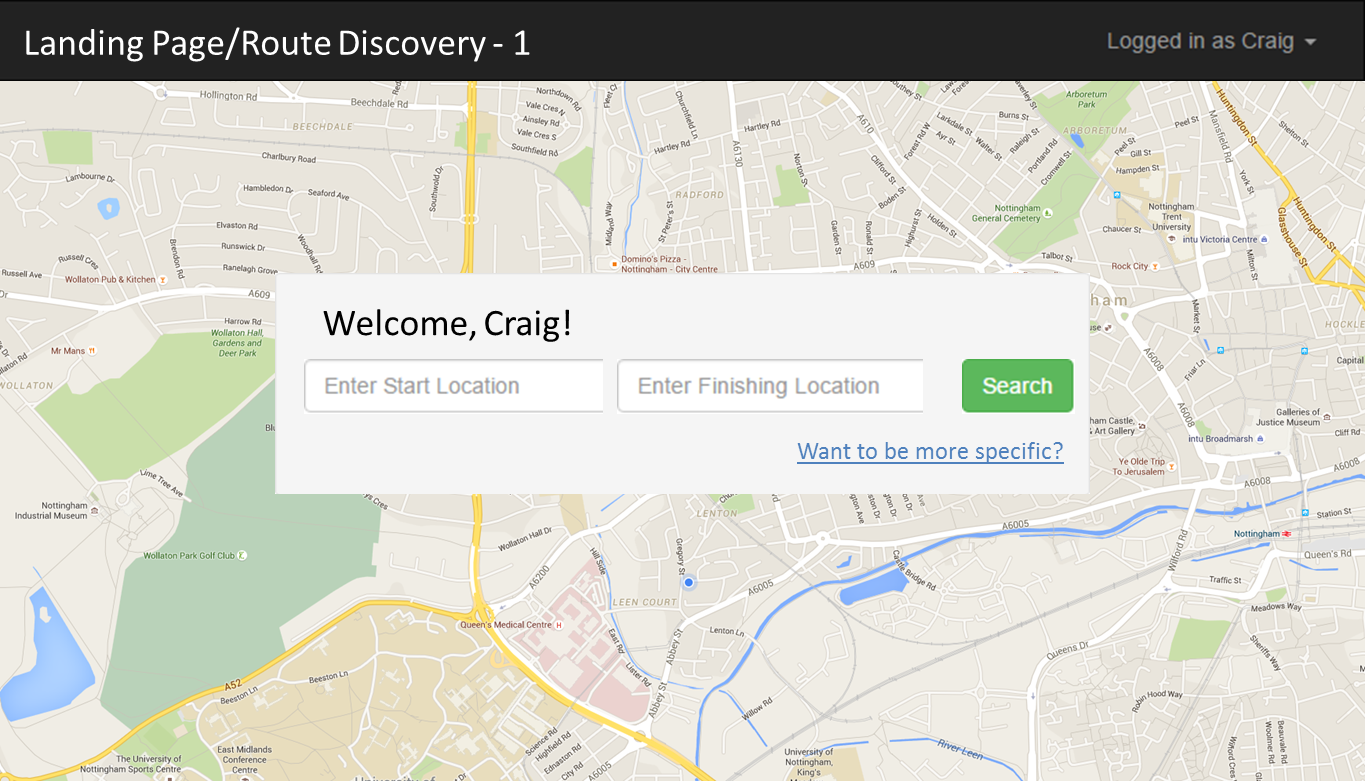
\includegraphics[width=0.725\textwidth]{images/appendix/landing1.png}
	\end{center}
	\vspace{-6mm}
\end{figure}

\begin{figure}[!ht]
	\begin{center}
		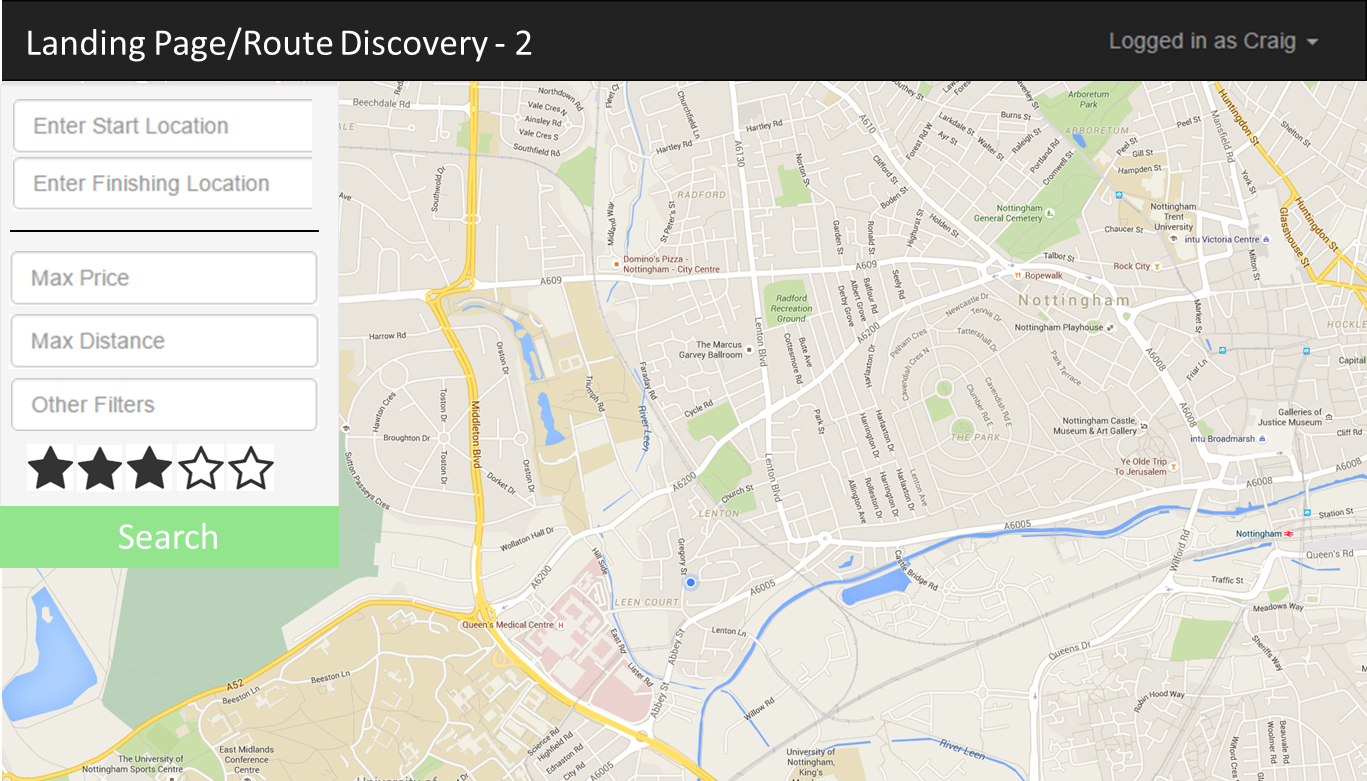
\includegraphics[width=0.725\textwidth]{images/appendix/landing2.png}
	\end{center}
	\vspace{-6mm}
\end{figure}

\begin{figure}[!ht]
	\begin{center}
		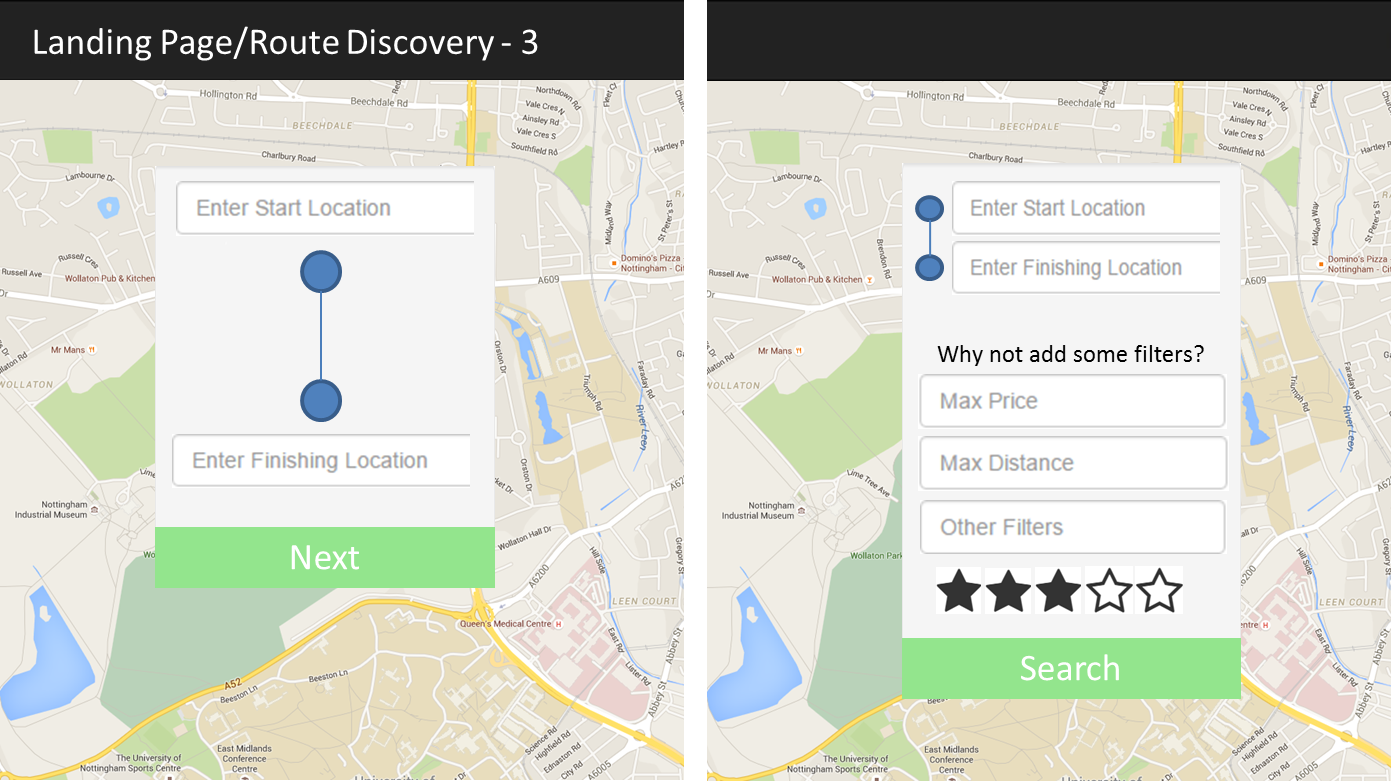
\includegraphics[width=0.725\textwidth]{images/appendix/landing3.png}
	\end{center}
	\vspace{-6mm}
\end{figure}

\newpage 
\subsection{Route Listing Page}
\begin{figure}[!ht]
	\begin{center}
		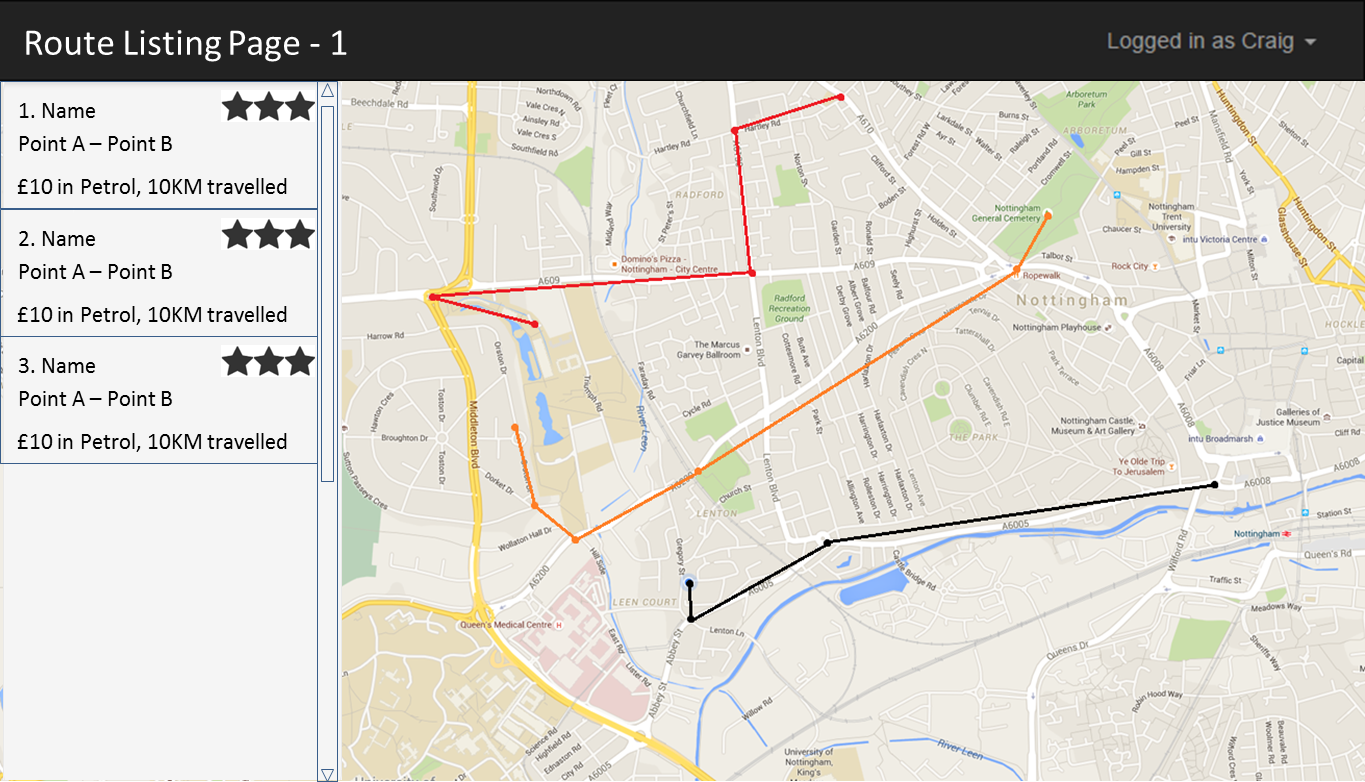
\includegraphics[width=0.75\textwidth]{images/appendix/rlp1.png}
	\end{center}
	\vspace{-6mm}
\end{figure}

\begin{figure}[!ht]
	\begin{center}
		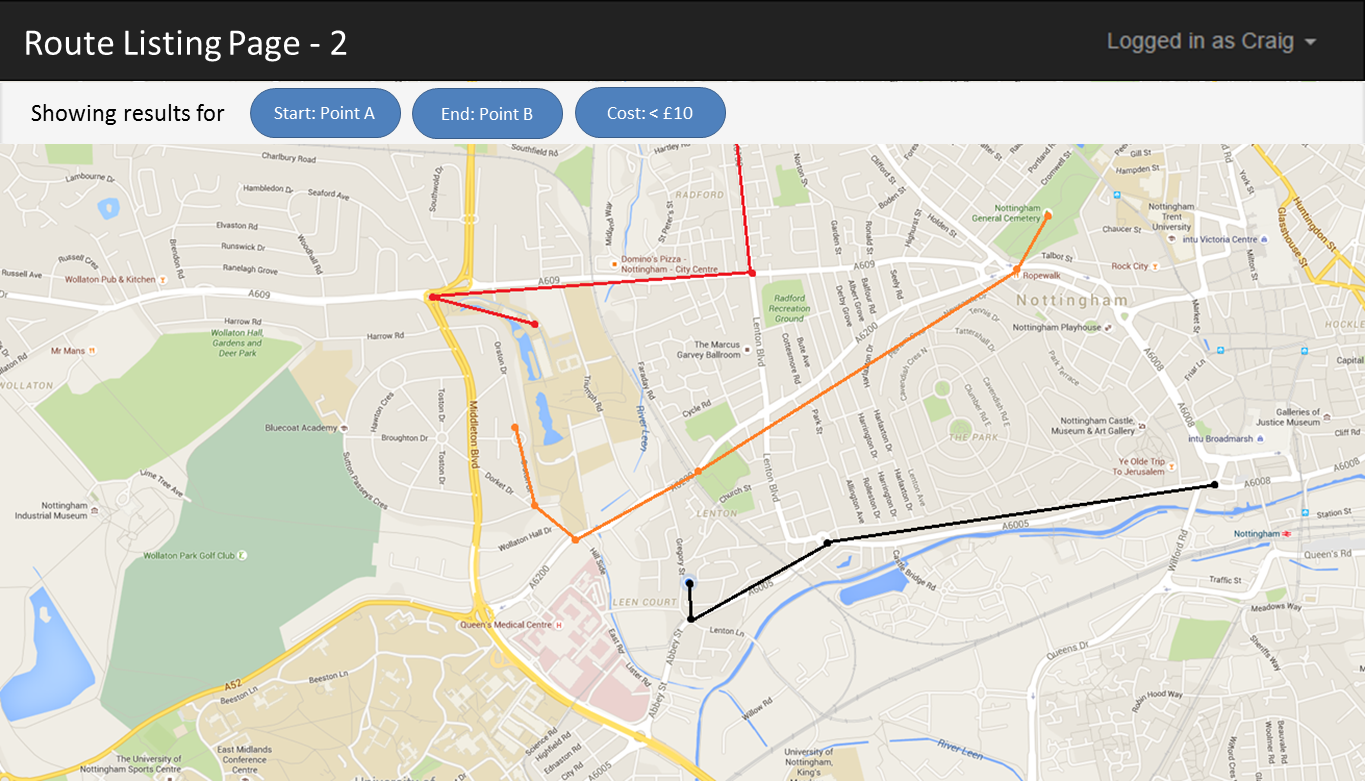
\includegraphics[width=0.75\textwidth]{images/appendix/rlp2.png}
	\end{center}
	\vspace{-6mm}
\end{figure}

\begin{figure}[!ht]
	\begin{center}
		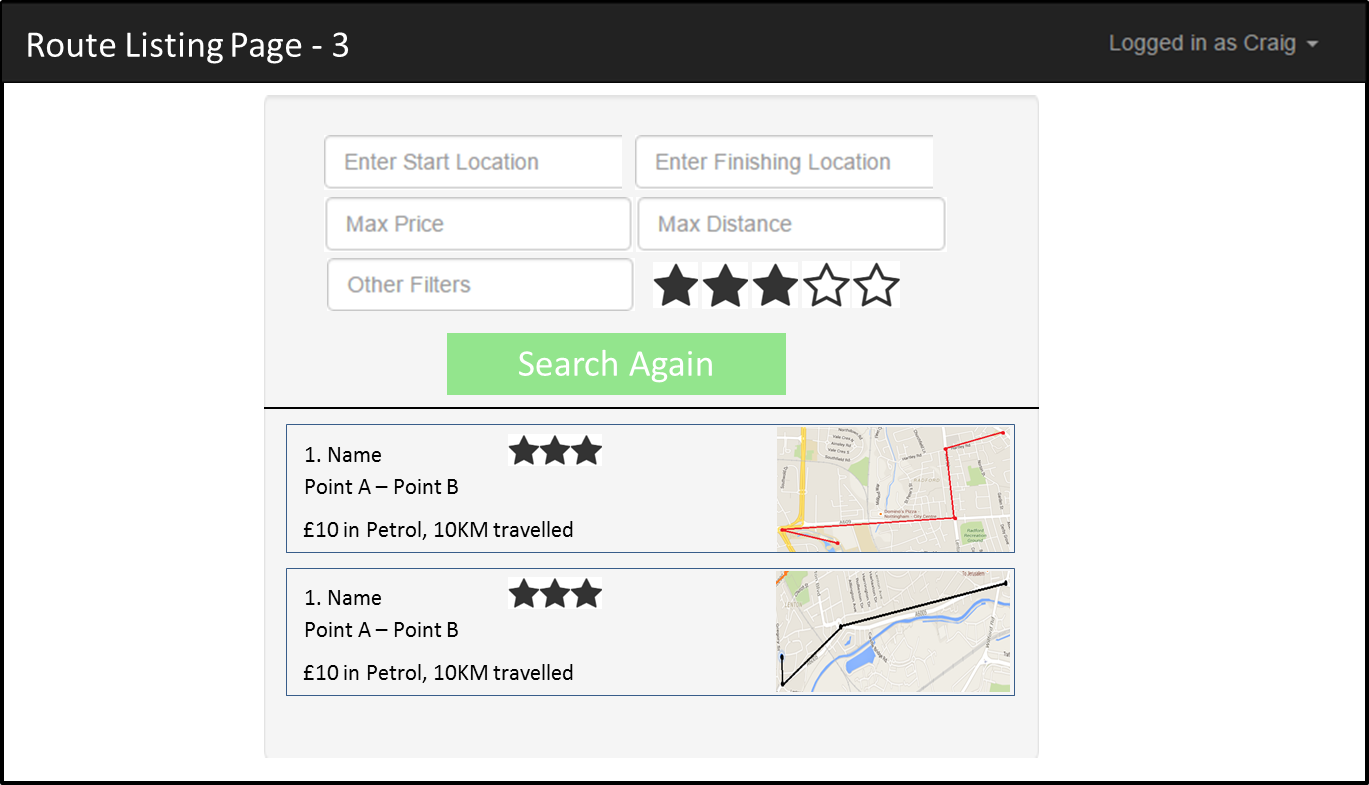
\includegraphics[width=0.75\textwidth]{images/appendix/rlp3.png}
	\end{center}
	\vspace{-6mm}
\end{figure}

\newpage 
\subsection{Route Detail Page}
\begin{figure}[!ht]
	\begin{center}
		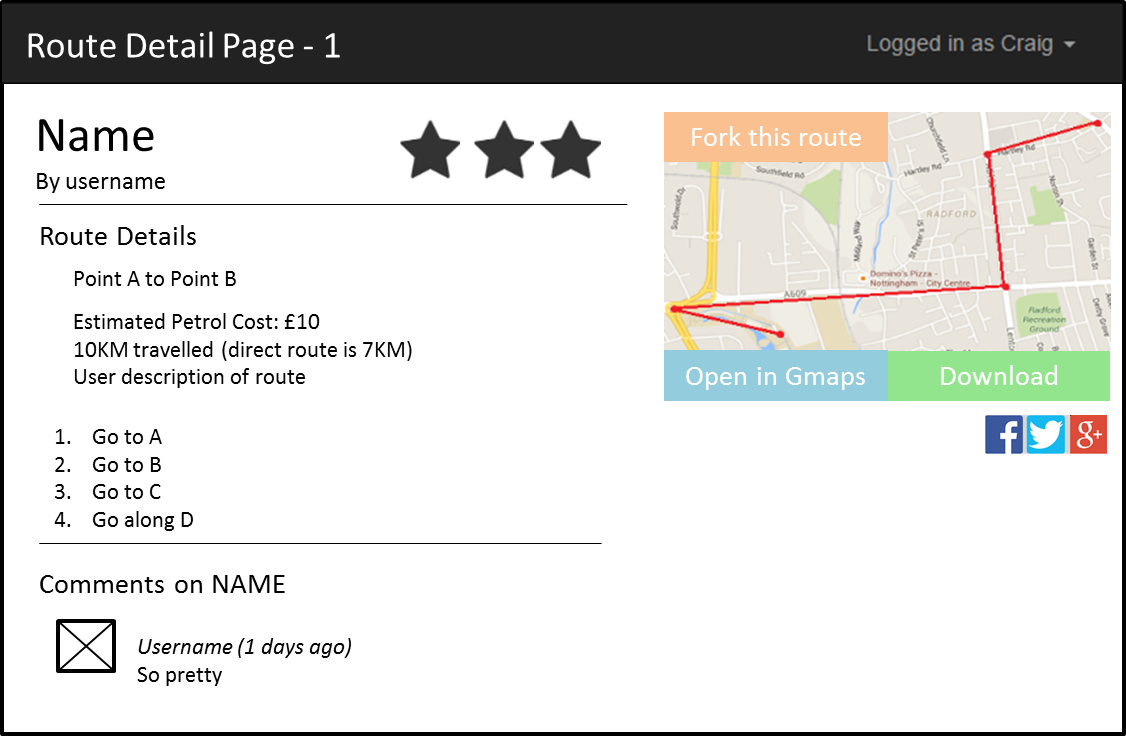
\includegraphics[width=0.75\textwidth]{images/appendix/rdp1.png}
	\end{center}
	\vspace{-6mm}
\end{figure}

\begin{figure}[!ht]
	\begin{center}
		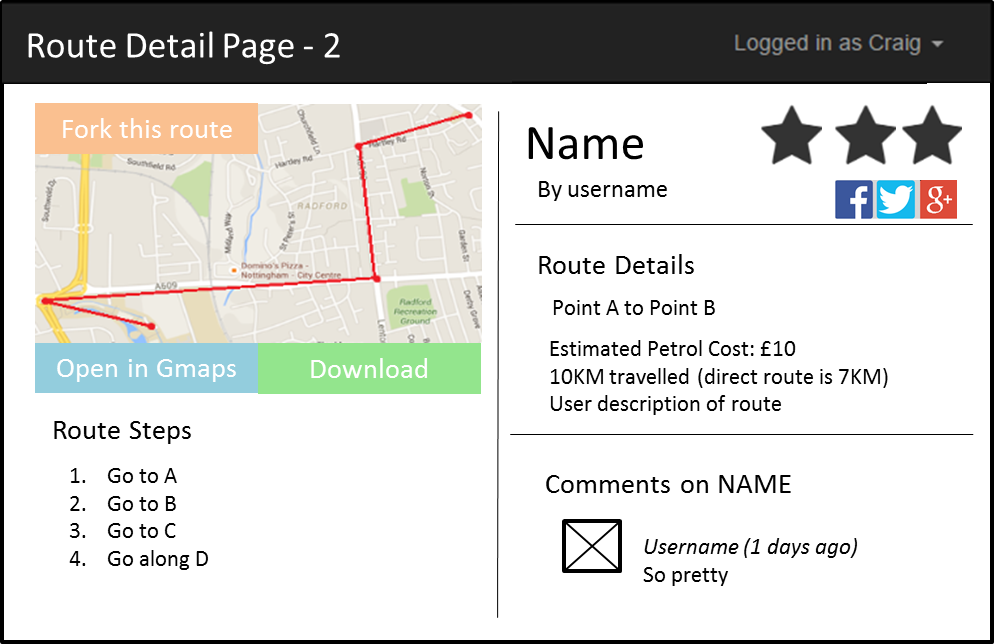
\includegraphics[width=0.75\textwidth]{images/appendix/rdp2.png}
	\end{center}
	\vspace{-6mm}
\end{figure}

\begin{figure}[!ht]
	\begin{center}
		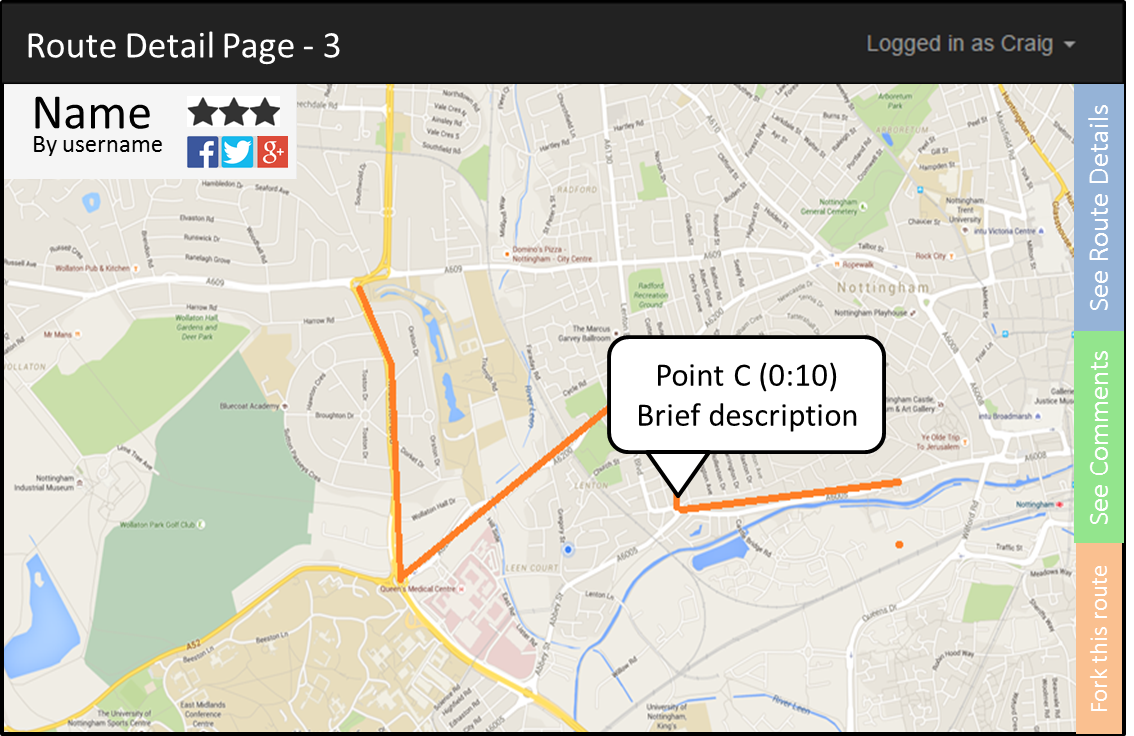
\includegraphics[width=0.75\textwidth]{images/appendix/rdp3.png}
	\end{center}
	\vspace{-6mm}
\end{figure}

\subsection{Route Creation Page}
\begin{figure}[!ht]
	\begin{center}
		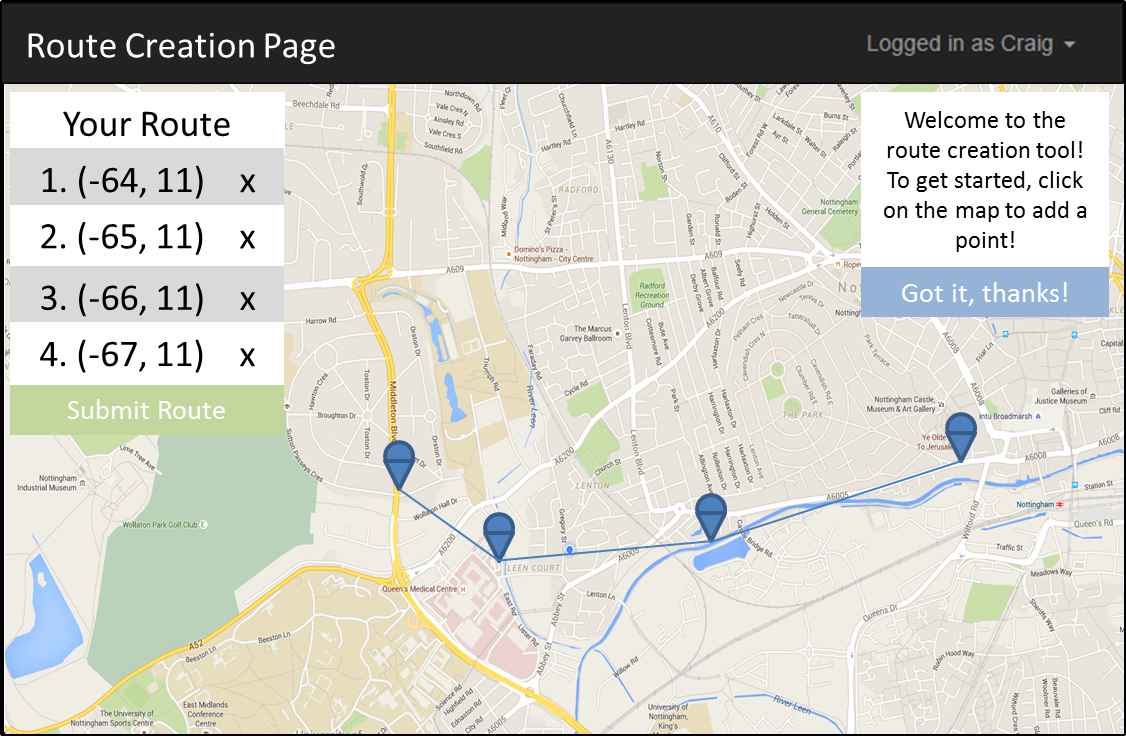
\includegraphics[width=0.8\textwidth]{images/appendix/rcp1.png}
	\end{center}
	\vspace{-6mm}
\end{figure}

\subsection{Profile Page}
\begin{figure}[!ht]
	\begin{center}
		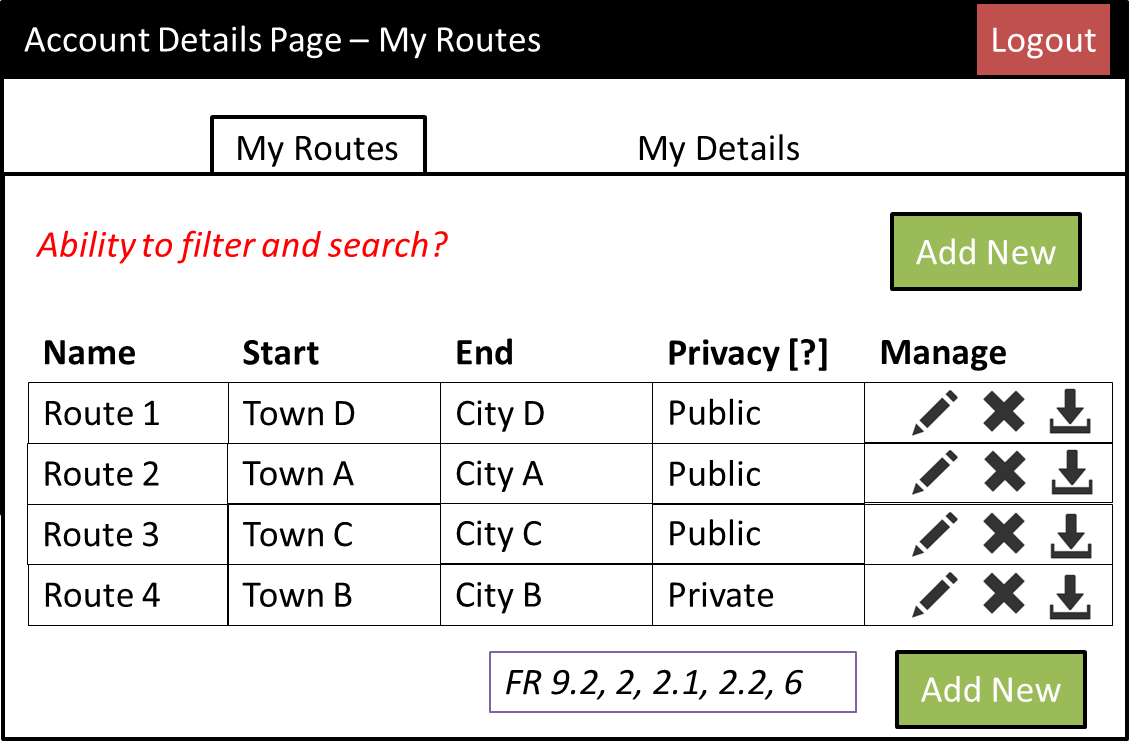
\includegraphics[width=0.8\textwidth]{images/appendix/prof1.png}
	\end{center}
	\vspace{-6mm}
\end{figure}


\newpage 
\section{Interface Design Heuristics}
\label{sec:idh}

\subsection{Jakob Nielsen's Usability Heuristics}
\begin{enumerate}
	\item Visibility of system status
	\item Match between system and the real world
	\item User control and freedom
	\item Consistency and standards
	\item Error prevention
	\item Recognition rather than recall
	\item Flexibility and efficiency of use
	\item Aesthetic and minimalist design
	\item Help users recognize, diagnose, and recover from errors
	\item Help and documentation
\end{enumerate}

\subsection{Ben Schneiderman's Golden Rules}
\begin{enumerate}
	\item Strive for consistency.
	\item Enable frequent users to use shortcuts.
	\item Offer informative feedback.
	\item Design dialog to yield closure.
	\item Offer simple error handling.
	\item Permit easy reversal of actions.
	\item Support internal locus of control.
	\item Reduce short-term memory load.
\end{enumerate}



